
\section{Systematic Literature Survey and Mapping}
\label{sec:survey}

\begin{figure}[htb]
        \centering
	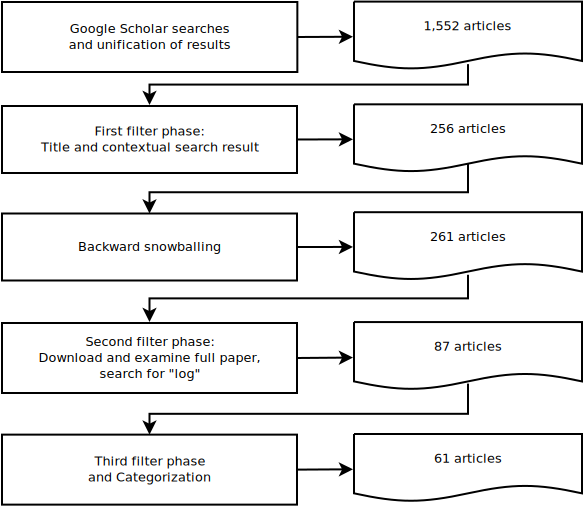
\includegraphics[width=\columnwidth, clip]{img/lit_survey.pdf}
	\caption{Our literature selection process, following \cite{petersen2015guidelines}.}
	\label{fig:lit-survey}
\end{figure}

% TODO (Caro): Integrate Petersen's guidelines
From our own experience, we know that the field of analyzing build
logs is relatively young, with perhaps the work on TravisTorrent the
most cited and central one. We also know there have been scattered
research efforts on build log analysis prior to it, mostly where the
log analysis was a side-part of the article. To the best of our
knowledge, there has not been an attempt to systematically overview
and survey them, despite their forseeable future and current importance.

\subsection{Study Selection}
% TODO shorten
\Cref{fig:lit-survey} presents an overview of our study selection.
In this first literature overview study on analyzing build logs, we
therefore want to survey as broad a population of scientific material
as possible. Note that we do not limit our sources to specific
Software Engineering venues, as is often done, but survey all sources
monitored by Google Scholar, including Bachelor's and Master's theses,
academic slide decks, and books. We use Google Scholar as opposed to
Scopus or other databases, as it is the search engine for acdemic
articles with the broadest and most current index, including preprints
from sources such as arXiv. One challenge is that no common
nomenclature has been established yet (in fact, this is one of the
goals of this article).

% TODO Caro cite guidelines
Since we cannot take for granted that ``analyzing build logs'' is the
cannonical term that other, isolated works have used, we instead
decdided to leave out the potentially variable ``analysis'' part and
instead focus on variations of the term ``build log''. This has the
advantage of being biunique: We explicitly decided to exclude systems
or event logs (see \Cref{sec:rw}). On the other hand, a Google Scholar
search for ``build log'' returns more than 2.2 million results
(2020-03-15). We therefore refined our search criterions for the four
different spelling possibilities of ``build log'' to exclude obvious
non-related works. This left us with 1,552 combined search results
(2020-03-15). The full search queries are documented in our replication
package~\cite{brandt2020chunk-replication}.

To make handling so many search results feasible, we employed a
two-pass filtering strategy:

First, we filtered out articles based on 1) their title and 2) the
contextual information Google Scholar displayed. We inlcuded only
publications written in a language intelligible to the authors (that
is, English or German), but only disregarded fewer than 1\% of search
hits due to this criterion. Our strategy was to err on the side of
caution, that is rather including a paper than not. We then unified
the results of the four search queries based on the link as the
identifying element, removing 60 articles that appeared in more than
one search query. We noticed that some publishers (ACM, Springer,
Google Books) augment a link to an article with a cutomized ID, which
specifies the link source ({\tt casa\_token, oid}). \todo{overly specific?} We automatically
removed it to find all true duplicates. After this process, we were
left with 259 (17\%) of the original search results.

With these 259 remaining articles, we followed a backward snowball
sampling for related work. This added three papers (five before
duplicate elimination) to our literature set, coming to a total of 261
articles. % TODO: update numbers

On the surviving artciles, we did a second filter phase by downloading the
full articles, reading their abstracts, and searching the full text
for the occurrence of ``log''. If these papers showed traces of
working with build logs, we included them in our survey. For the
snowballed set, we included two of the three articles, both of which
stem from the same first author, were borderline-includes, and had
called build logs from the Linux kernel ``build traces.'' In total, we
were left with 90 articles after this search.

\subsection{Article Classification}
Having trimmed down the set of articles, we investigated them in depth.
kept all articles that use logs from software builds as input to some kind of process.
we wanted to characterize how researchers use buildlogs as input to any processes.
Interesed in 
\begin{itemize}
  \item what kind of build logs they are using and the source of these logs.
  \item what information they are retrieving from the logs, 
  its kind (chunk/classification) and 
  what they use the retrieved information for
  \item which technique they are using to process the build logs,
  in how much detail it is described and whether they published their tools
\end{itemize}
To objecifiy our data extraction we created a template of the targeted factors
and performed a pilot on five articles. Two authors extracted the data from the
five pilot articles and we held a consensus meeting to unify our understanding
of the factors in the data extraction templates. The remaining articles were
divided over these two authors. We inspected the articles as closesly as necessary,
starting from occurences of ``log'' or ``build'' within the text.
The full data extraction template and our results of this step can be found in
our replication package \todo{cite}.

In this pass we further identified x duplicate articles \todo{do we push those to the last pass?}.
For several cases, multiple articles extended others, though still reported on
the same work with the respect to analyzing build logs.
Of these we only considered the earliest article which reported on the processing
of build logs.

\subsection{Results}
lots of:
- categories + frequencies of answers

\subsubsection{Retrieved Information}

\subsubsection{Retrieval Technique}

\subsubsection{Build Logs}

\subsection{Discussion}
various researchers analyzing build logs to support their research,
tools developed to help developers \todo{motivational reference}.

\subsubsection{Retrieved Information}
why from build logs? not avaliable in cleaner format much use for
research, a bit of developer information / tools following: research
so many logs that unfeasible to do manually, less focus on tools for
devs (caveat! we excluded books and documentation on industrial tools
-> many approaches there to make build logs digestible, tough many
focus on general minimizing of the data presented, not retrieving
specific chunks)

\subsubsection{Retrieval Technique}
broadly mentioned shortly, rarely explained in detail we follow that
researchers often see this as an unimportant side fact work needed to
be done to get the big work done

\subsubsection{Build Logs}
often focussed on specific logs, sometimes mentioned because of effort
developing a parser other times also because other tools used in
further research are limiting the scope (reference paper with PIT
tool). many focus on maven because of it's prevalence also in respect
to other tools much research done on travis ci logs b/c of their
abundance and open availability

